\documentclass[runningheads]{llncs}

\usepackage{amssymb}
\setcounter{tocdepth}{3}
\usepackage{graphicx}
%%%%
\usepackage{color}
\usepackage{alltt}
\usepackage{verbatim}
\usepackage[utf8]{inputenc}
\usepackage[spanish]{babel}
%%
\usepackage{url}
\urldef{\mailsa}\path|{pgarcia,pedro}@atc.ugr.es|

\newcommand{\keywords}[1]{\par\addvspace\baselineskip
\noindent\keywordname\enspace\ignorespaces#1}

\begin{document}
 \pagestyle{empty} %ESTO QUITA LOS NÚMEROS DE PÁGINA
\mainmatter  % start of an individual contribution

% first the title is needed
\title{Estudio sobre algoritmos genéticos en la nube y el modelo de programación MapReduce\thanks{Financiado con los proyectos EvOrq (TIC-3903) y Beca FPU AP2009-2942. }}

% Mete tambi?n el del ministerio, que estaba vigente cuando el PFC. 

% a short form should be given in case it is too long for the running head
\titlerunning{Estudio sobre AGs en la nube}

% the name(s) of the author(s) follow(s) next
%
% NB: Chinese authors should write their first names(s) in front of
% their surnames. This ensures that the names appear correctly in
% the running heads and the author index.
%
\author{G. Mu\~noz \inst{1} \and Pablo Garc\'ia-S\'anchez\inst{1}  \and Pedro A. Castillo\inst{1}  \and Quien sea \inst{1}}
%
\authorrunning{P. Garc\'ia-S\'anchez et al.}
% (feature abused for this document to repeat the title also on left hand pages)

% the affiliations are given next; don't give your e-mail address
% unless you accept that it will be published
\institute{Dept. de Arquitectura y Tecnología de los Computadores, Universidad de Granada\\
\mailsa}


%
% NB: a more complex sample for affiliations and the mapping to the
% corresponding authors can be found in the file "llncs.dem"
% (search for the string "\mainmatter" where a contribution starts).
% "llncs.dem" accompanies the document class "llncs.cls".
%

\toctitle{Estudio sobre algoritmos genéticos en la nube y el modelo de programación MapReduce}
\tocauthor{Authors' Instructions}
\maketitle


\begin{abstract}
Este trabajo presenta el proyecto fin de carrera Estudio sobre algoritmos genéticos en la nube y el modelo de progrmación MapReduce.

\end{abstract}


\section{Introducción}
\noindent En la última década Internet ha transformado nuestra economía y nuestra sociedad. Ha demostrado ser una infraestructura de comunicación 
y enlace de gran valor que se adapta gradualmente a las necesidades de los usuarios. Con Internet se ha creado una red mundial de 
intercambio de conocimientos, creatividad y colaboración. 

Del mismo modo, Internet ha dado un gran salto adelante gracias al despliegue de la banda ancha de muy alta velocidad, lo que ha 
permitido el lanzamiento de muchos nuevos servicios interactivos y de contenido. 

Todo esto hace que los programas informáticos ofertados en la red como un servicio disminuyan sus costes y aumenten su eficacia, 
provocando una gran mejora de la productividad. Desplegado adecuadamente, el llamado Internet del futuro, que cada vez es más 
presente, trae consigo innovación, aumento de la productividad, nuevos mercados y más crecimiento y empleo en esta década que 
recién acabamos de comenzar. 

En este marco se engloba el Cloud Computing, un nuevo modelo de negocio en Internet, que beneficia tanto al proveedor de 
servicios en la nube como al usuario, capaz de tener acceso instantáneo a una infraestructura barata, escalable y fácilmente 
accesible. 
 
Paralelamente a esta transformación, la ciencia ha estado evolucionando constantemente durante los últimos lustros, en gran parte, 
gracias al uso  de la tecnología. La investigación científica avanza al unísono con ésta, pues un cambio tecnológico, la mayoría 
de las veces, abre un nuevo abanico de posibilidades para la comunidad científica, puesto que, independientemente de que se trate 
de investigación y desarrollo en un ámbito clínico, científico o industrial, existen múltiples parámetros, como el uso intensivo 
de tecnologías y procesamiento de datos, que son comunes e independientes del sector en el que se desarrollen. 

Dentro de la investigación existe además en los últimos tiempos un crecimiento exponencial del volumen de datos necesario para 
resolver los cada vez más complejos problemas presentes en el día a día de un científico o investigador. Dentro de estos conjuntos 
de problemas se encuentran los de búsqueda, a menudo representados por medio de Algoritmos Genéticos, que se usan cada vez más en 
escenarios de gran complejidad. 


Sentando estos principios evidentes en la sociedad actual, el motivo de este trabajo es el de buscar una aproximación nueva para 
desarrollar trabajos de investigación usando las facilidades que nos brinda el Cloud Computing, y concretamente la resolución de 
problemas de búsqueda representados mediante algoritmos Genéticos, yendo más allá y sentando las bases de un framework como 
Hadoop Map Reduce, para la reducción de complejidad y tiempo en estos fines.



\section{Cloud Computing}

Cloud computing es aún un paradigma en evolución, sus definiciones, arquitecturas, modelos, casos de uso, tecnologías base, problemas, 
riesgos y beneficios, son continuamente redefinidos en debates promocionados por el sector público y privado. En\cite{Bible2011} 
podemos ver varias  definiciones aunque muchos citan como más precisa la definición dada por el NIST, se enuncia a continuación.
Según el NIST (National Institute of Standards and Technology) podemos definir el Cloud Computing como: 

\textit{Cloud Computing es un modelo para habilitar acceso conveniente por demanda a un conjunto compartido de recursos computacionales 
configurables, por ejemplo, redes, servidores, almacenamiento, aplicaciones y servicios, que pueden ser rápidamente proporcionados y 
liberados con un esfuerzo mínimo de administración o de interacción con el proveedor de servicios. Este modelo de nube promueve la 
disponibilidad y está compuesto por cinco características esenciales, tres modelos de servicio y cuatro modelos de despliegue. }



En un intento de adentrarse en lo que es y no es el Cloud computing compararemos este paradigma con la computación tradicional, 
que ha habido hasta este tiempo. Con la computación tradicional ejecutamos copias de software en cada ordenador. 
Los documentos que creamos  son almacenados en el ordenador en el que fueron creados. Aunque se puede acceder a los documentos desde 
otros ordenadores de la red, no se puede desde ordenadores de fuera de ella. 

Con cloud computing, los programas que usamos no se ejecutan en nuestro ordenador personal, sino que son almacenados en servidores 
accedidos vía Internet. Si tu ordenador se rompiera, el software seguiría estando operativo para los demás. De la misma forma se hace 
para los documentos que creamos; son almacenados en una colección de servidores. Cualquiera con permiso puede, no sólo acceder a los 
documentos, sino también editar y colaborar en dichos documentos en tiempo real. A diferencia de la computación tradicional, el modelo 
de cloud no es PC-Céntrico. El dispositivo que se usa para acceder a la información no es lo más importante. A continuación, veremos 
qué es Cloud Computing y qué no es \cite{Web08} .

\subsection{Qué no es cloud computing}

Cloud computing no es una red de ordenadores. Con una red, las aplicaciones  y documentos son almacenados en un servidor de la empresa 
y accedidos a través de la red de la empresa. Cloud computing es mucho más que esto. Engloba múltiples empresas, múltiples servidores y 
múltiples redes. A diferencia de una red de ordenadores, los servicios cloud y el almacenamiento pueden ser accedidos desde cualquier 
ordenador del mundo con una conexión a internet. 

Cloud computing tampoco es la subcontratación de un servicio externo de manera tradicional, donde la compañía contratada presta sus 
servicios a la empresa contratadora. Mientras una empresa de outsourcing organiza sus datos y aplicaciones, estos documentos y 
programas solamente son accesibles a los empleados de la empresa a través de la red de la misma, no a todo el mundo vía internet.
Así que, a pesar de las aparentes similitudes, las redes y el outsourcing no son cloud computing.


\subsection{Qué es cloud computing}

La clave de la definición de Cloud Computing es el Cloud en sí mismo. Para nuestro propósito, el cloud es un gran conjunto de ordenadores 
interconectados. Estos computadores pueden ser PC's o servidores, públicos o privados. 

Esta nube de computadores se extiende más allá de una simple compañía o empresa. Las aplicaciones y datos servidos por la nube están 
disponibles para un amplio grupo de usuarios, a través de empresas y plataformas. El acceso es vía Internet. Cualquier usuario autorizado 
puede acceder a estos documentos  y aplicaciones  desde cualquier ordenador con conexión a Internet. Y, para el usuario, la tecnología e 
infraestructura que se esconde detrás de la nube es invisible. 



En general, como vemos en la figura\ref{Figura3} Cloud computing surge de la combinación y agrupación de tecnología ya conocidas, que 
permiten obtener un nuevo enfoque y proyección.


Para ejemplificar algunos de los puntos más interesantes del cloud computing nos basaremos en Google, una de las principales 
compañías impulsoras del Cloud. Según su perspectiva, hay seis propiedades clave en el cloud computing.

\begin{itemize}

\item Es ``User-Centric'': Una vez que tú eres un usuario conectado a la nube, cualquier cosa que haya almacenada allí - documentos, mensajes, 
imágenes, aplicaciones - se convierte en tuya. Además, no solo los datos son tuyos sino que puedes compartirlos con otros. 
En efecto, cualquier dispositivo que acceda a tus datos en la nube también convierte los datos en suyos.
\item Es ``Task-Centric'': En vez de concentrarse en la aplicación y qué hacer, se centra en lo que necesitas y cómo la aplicación puede 
hacerlo por ti. Las aplicaciones tradicionales - procesadores de textos, hojas de cálculo, email... -  se están convirtiendo en más 
importantes que los documentos que se crean.
\item Es poderoso: Conectando cientos o miles de computadores juntos en una nube se crea una riqueza de computación imposible de hacer 
en un único PC.
\item Es accesible: Como los datos son almacenados en la nube, usuarios pueden recuperar información instantáneamente desde múltiples 
repositorios. No estás limitado a una única fuente de datos, como lo estás en un PC.
\item Es inteligente: Con el volumen de datos almacenados en la nube, el data-mining y análisis son necesarios para acceder a esta 
información de una manera inteligente.
\item Es programable: Muchas de las tareas necesarias para el cloud computing deben de ser automatizadas. Por ejemplo, para proteger 
la identidad de los datos, la información almacenada en un único computador en la nube debe ser replicada en los otros computadores 
de la nube. Si uno de éstos falla, la programación de la nube redistribuirá automáticamente los datos de éste computador hacia uno 
nuevo de la nube.

\end{itemize}

\section{Algoritmos Genéticos}


La técnica de búsqueda conocida como Algoritmo Genético se basa en los mecanismos de selección que utiliza la naturaleza, 
de acuerdo a los cuales los individuos más aptos de una población son los que sobreviven, al adaptarse más
fácilmente a los cambios que se producen en su entorno. Hoy en día se sabe que estos cambios se efectúan en los genes de 
un individuo (unidad básica de codificación de cada uno de los atributos de un ser vivo), 
y que sus atributos más deseables (es decir, los quele permiten adaptarse mejor a su entorno) se transmiten a sus descendientes 
cuando éste se reproduce sexualmente. 

La primera mención del término Algoritmo Genético, y la primera publicación
sobre una aplicación del mismo, se deben a J.D.Bagley \cite{Bagley67}, que diseñó AGs para
buscar conjuntos de parámetros en funciones de evaluación de juegos. 
Pero es otro científico el considerado creador de los AGs: John Holland, que los desarrolló, junto a sus alumnos y colegas, 
durante los 60 y 70.  

El propósito original de Holland no era diseñar algoritmos para resolver problemas concretos, sino estudiar, de un modo formal, 
el fenómeno de la adaptación tal y como ocurre en la naturaleza y desarrollar vías de extrapolar esos mecanismos de adaptación
natural a los sistemas computacionales.  

En \cite{Holland75} Holland presentaba el AG como una
abstracción de la evolución biológica, y proporcionaba el entramado teórico para la adaptación bajo el algoritmo genético. 
El AG de Holland era un método para desplazarse, de una población de cromosomas a una nueva población, utilizando
un sistema similar a la selección natural junto con los operadores de cruce, mutación e inversión inspirados en la genética. 
En este primitivo algoritmo, cada cromosoma consta de genes (bits) y cada uno de ellos es una muestra de un alelo particular (0 ó 1). 
El operador de selección escoge entre los cromosomas de la población aquellos con capacidad de reproducción, y entre éstos, 
los que sean más compatibles producirán más descendencia que el resto. El operador de cruce extrae partes de dos cromosomas,
imitando la combinación biológica de dos cromosomas aislados (gametos). Y por último, el operador de mutación se encarga de cambiar, 
de modo aleatorio, los valores del alelo en algunas localizaciones del cromosoma. 


\section{Fundamentos biológicos}

La computación evolutiva, dentro de la que se encuadran los AGs, tiene una fuerte base biológica. Originalmente, 
los algoritmos evolutivos consistían en copiar procesos que tienen lugar en la selección natural. A pesar de que 
aún hoy en día no todos los detalles de la evolución biológica son completamente conocidos, existen algunos hechos apoyados 
sobre una fuerte evidencia experimental:

\begin{itemize}
 \item La evolución es un proceso que opera, más que sobre los propios organismos, sobre los cromosomas. Estos cromosomas son 
 partes del ADN portadores de los factores de la herencia o genes.
 \item La selección natural es el proceso por el cual los organismos mejor adaptados desplazan lentamente organismos peor adaptados. 
 Este proceso conduce a la acumulación lenta de cambios genéticos favorables en una población. Dicha selección al operar a lo 
 largo de muchas generaciones puede cambiar los atributos básicos de la población original de organismos.
 \item Los procesos evolutivos tienen lugar durante la etapa de reproducción. Aunque existe una larga serie de mecanismos 
 que afectan a la misma, los más comunes son la mutación y el cruce o recombinación.
\end{itemize}


En analogía analogía directa con el comportamiento natural, los AGs trabajan con una población de individuos, cada uno de los cuales 
representa una posible solución a un problema dado. A cada individuo se le asigna un valor o puntuación, relacionado con la bondad 
de dicha solución, llamado fitness. En la naturaleza, esto equivaldría al grado de efectividad de un organismo para competir por 
unos determinados recursos. Cuanto mayor sea la adaptación de un individuo al problema, mayor será la probabilidad de que el mismo 
sea seleccionado para reproducirse, cruzando su material genético con otro individuo seleccionado. Este cruce producirá nuevos 
individuos -descendientes de los anteriores- los cuales comparten algunas de las características de sus padres. Cuanto
menor sea la adaptación de un individuo, menor será la probabilidad de que dicho individuo sea seleccionado para la reproducción, 
y por tanto de que su material genético se propague en sucesivas generaciones posteriores. De esta manera se produce una nueva población
de posibles soluciones, la cual reemplaza a la anterior y verifica la propiedad de contener una mayor proporción de buenas 
características en comparación con la población anterior. Así a lo largo de las generaciones las buenas características se
propagan a través de la población.  Si el AG ha sido bien diseñado, la población convergerá hacia una solución óptima del problema.

Según \cite{Enfoque09} estas ideas están enla base del diseño de los algoritmos evolutivos. Además, muchas de las propiedades de la
evolución de los seres vivos, como la edad, la mayor o menor tendencia a la mutación según el estadio de la evolución, etc. están
siendo objeto de investigación para su incorporación a las técnicas de computación evolutiva. Sin embargo, los algoritmos evolutivos
no tratan de ser un reflejo fiel de la evolución biológica. Debemos tener en cuenta que la naturaleza evoluciona a lo largo de millones
de años, mientras que a nosotros nso interesa que nuestros algoritmos nos proporcionen una solución en un tiempo algo más corto.



\section{Algoritmo Genético Básico}

En esta sección se describen los componentes de un algoritmo genético básico y sus formas más comunes.

\subsection{Representación de los Individuos}

Desde los primeros estudios de los AGs los individuos son cadenas binarias, siendo hoy en día aún la aproximación
más utilizada, aunque existen otras que utilizan letras o valores númericos para representar a sus cromosomas. 
Podemos ver un ejemplo en la \ref{Figura9}


La sencillez de la representación binaria que utilizan los AGs les aporta características muy importantes de eficiencia. 
Sin embargo debemos disponer de un método para poder evaluar la adecuación del individuo como solución al 
problema. Lógicamente, el método de transformación es específico del problema considerado. Sin embargo, a la hora de diseñar
el método de codificación es importante tener en cuenta una serie de directrices. Así, debemos buscar una codificación tal que
cada punto del espacio de búsqueda esté representado por el mismo número de cadenas binarias, y tal que sea capaz de representar
todos los puntos del espacio del problema. 

En el contexto de los AGs, el término cromosoma se refiere a un candidato a solución del problema, que frecuentemente es 
codificado como una cadena de bits. Los genes son tanto un bit como bloques cortos de bits adyacentes 
que codifican un elemento particular del candidato a solución. Un alelo en una cadena de bits será 
un 0 o un 1 (para alfabetos largos cada posición puede tener más alelos). El genotipo de un individuo en un AG que emplea
cadenas de bits es, simplemente, la configuración de bits del cromosoma de ese individuo. 

Cabe resaltar que en este trabajo usaremos tanto codificación binaria como codificación real que
consiste en exactamente lo mismo pero un gen es representado como un número real, generalmente en un dominio dado por el 
problema. 


\subsection{Funcionamiento}

Sea X el problema a resolver, el esquema general de un algoritmo genético es el siguiente \cite{Her03}:




A continuación se procederá a una explicación exhaustiva de dicho algoritmo.
Dada una representación de candidatos a soluciones en una cadena de bits, un AG simple, tal y como 
se describe en \cite{Mit98}, funcionaría del siguiente modo:

\begin{enumerate}
 \item Comenzar con una población P generada aleatoriamente de n cromosomas de L bits.
 \item Calcular el valor de la función de evaluación o fitness (f(x)) para cada cromosoma x de P.
 \item Repetir los siguientes pasos hasta que se hayan creado todos los  descendientes:
 \begin{enumerate}
    \item Seleccionar un par de cromosomas de P, siendo la probabilidad de selección proporcional al fitness.
    Los cromosomas seleccionados serán llamados cromosomas padre.
    \item Con probabilidad \textit{$p_c$} (tasa de cruce), cruzar el par de cromosomas padre en un punto (o más)
    elegido aleatoriamente para formar dos descendientes. Si no tiene lugar ningún cruce, formar dos descendientes que sean copias
    exactas de sus respectivos padres.
    \item Mutar los dos descendientes en cada lugar con probabilidad \textit{$p_m$} (tasa de mutación), y colocar 
    los cromosomas resultantes en la nueva población P'.
 \end{enumerate}
 \item Reemplazar la población actual P con la nueva población P'.
 \item Evaluar la condición de finalización.
 \item Volver al paso 2.

\end{enumerate}

En el paso 2 del algoritmo se habla de una función de evaluación, la cual debe ser diseñada para cada problema de manera 
específica. Dado un cromosoma cualquiera, la función de evaluación le asigna un número real, que se supone refleja el nivel de 
adaptación al problema del  individuo representado por el cromosoma. 

Asimismo, la primera operación del paso 3 del algoritmo es la llamada fase de selección. Esta selección se efectúa usando 
un procedimiento que favorezca a los individuos mejor adaptados. Existen diferentes métodos de selección, que posteriormente
veremos. 

Cada iteración de este proceso recibe el nombre de generación.
Cada generación se obtiene a partir de la anterior por medio de los llamados operadores de reproducción (paso 3 del algoritmo), 
que pueden ser de dos tipos:

\begin{enumerate}
 \item \textbf{Copia:} Es un tipo de reproducción asexual, en la que un determinado número de individuos pasa directamente a la 
 siguiente generación, sin sufrir ningún proceso de variación en sus genes.
 \item \textbf{Cruce:} Es una reproducción de tipo sexual en la que se genera una descendencia a partir de un número fijo de 
 individuos, dos por lo general, de la generación anterior. Existen varios tipos de cruce, que veremos más tarde.
\end{enumerate}


El algoritmo acabará cuando se cumpla la condición de fin, que normalmente será una de las siguientes:

\begin{enumerate}
 \item Se ha encontrado una solución que satisface un criterio mínimo.
 \item Se ha llegado a un número determinado de generaciones establecido previamente.
 \item Se ha llegado a un límite preestablecido en tiempo de computación.
 \item Tras varias generaciones el fitness de la mejor solución no ha variado.
 \item Parada manual.
 \item Combinación de las anteriores
\end{enumerate}

Posiblemente el criterio más utilizado sea el primero, según el cual De Jong en su tesis doctoral
\cite{John75} afirmó que si el AG es correcto, la población evolucionará a lo largo de las sucesivas generaciones de tal forma que la
evaluación media entre todos los individuos, así como la propia del mejor individuo, convergerán hacia el óptimo global. 
Se dice que un gen ha convergido cuando al menos el 95\% de los individuos de la población comparten el mismo valor para dicho gen. 
Se dice que la población converge cuando todos los genes han convergido. Se puede generalizar dicha definición al caso en que al menos un
$\beta \%$ de los individuos de la población hayan convergido. 

El esqueleto de este algoritmo es la base de la mayoría de las aplicaciones de los algoritmos genéticos. Se podría profundizar mucho más 
en detalles sobre cuales deben ser las diferentes probabilidades, tamaño de la población y número de generaciones. De esos detalles 
dependerá, en gran parte, el éxito o fracaso de nuestro algoritmo.



\section{Modelo MapReduce}


Durante años, los programadores se han visto forzados a realizar implementaciones específicas para trabajar con grandes 
volúmenes de datos en sus entornos distribuidos de trabajo.

Pese a que no siempre es necesario, el tamaño de la información entrante suele ser grande y los cálculos deben ser distribuidos 
entre una gran multitud de máquinas para acabar en un tiempo razonable. Los problemas de cómo paralelizar estos cálculos, 
distribuir la información y manejar los fallos dificultan basatante la labor de implementación. 

El modelo de programación MapReduce es una propuesta que pretende resolver las dificultades anteriores, ya que sus características 
y motivación se basan en la delegación de los cómputos intensivos en datos a un clúster de máquinas remotas que,
mediante un sistema de ficheros distribuido, repartirán la carga de trabajo, optimizando tiempo y recursos. 
Asimismo, facilita un patrón de desarrollo paralelo para simplificar la implementación de aplicaciones intensivas en 
datos en entornos distribuidos. Este modelo puede dividir un espacio grande de problema en espacios pequeños y paralelizar 
la ejecución de tareas más pequeñas en estos sub-espacios. 

Este modelo ha cobrado especial interés por su aplicabilidad en entornos de Cloud Computing \cite{Web08}. 
MapReduce ofrece unas ventajas muy directas y evidentes como es la centralización de los datos en servidores remotos, 
eliminando las dependencias con los soportes físicos; o la contratación de servicios en función de las
necesidades de las empresas, sin tener que añadir equipos, software o personal, lo que conlleva un considerable ahorro 
también en el plano energético. 

Este capítulo se estructura en varias secciones. En la primera de ellas se introduce el modelo MapReduce, desarrollando sus
dos primitivas fundamentales: map y reduce. En siguientes secciones se irán analizando las distintas implementaciones y 
ejemplos de uso, así como una visión general de Amazón Elastic MapReduce, la implementación de este paradigma por parte de
Amazon.

\section{Introducción}

MapReduce \cite{Dea08} es un modelo de programación, desarrollado por Google, que es utilizado para procesar grandes conjuntos de 
datos distribuidos a lo largo de un clúster de servidores. Este procesado computacional puede tener lugar tanto sobre datos
almacenados en sistemas de ficheros, como en bases de datos. El modelo de programación está inspirado en los lenguajes funcionales 
y permite al desarrollador expresar sus algoritmos utilizando únicamente dos funciones, \textbf{map} y \textbf{reduce}. 

Las funciones map y reduce de MapReduce se definen sobre datos estructurados en pares clave-valor. La función map, escrita por el 
usuario, recibe un par clave-valor y devuelve un conjunto de pares clave-valor intermedio:

%\begin{equation}
%	map: (k1 , v1) \xrightarrow{} [(k2 , v2)] 
%  \label{EcuacionMap}
%\end{equation}


Esta función (\ref{EcuacionMap})  se aplica en paralelo a cada par del conjunto de datos de entrada produciendo una lista de 
pares $(k2, v2)$ por cada llamada. MapReduce agrupa todos los valores intermedios asociados con la misma clave k y se los 
pasa a la función reduce.

La función reduce (\ref{EcuacionReduce}) recibe dicha clave y su conjunto de valores asociados y los fusiona para formar un conjunto 
de valores más pequeño:


%\begin{equation}
%	reduce: (k2 , [v2]) \xrightarrow{} [v3]
%	\label{EcuacionReduce}
%\end{equation}


Cada llamada reduce produce bien una lista v3 o un valor vacío. Los resultados de las llamadas se recopilan en la lista de 
resultados buscada. 




Desde la perspectiva del flujo de datos, la ejecución de MapReduce consiste en M tareas map y R tareas reduce independientes. 
Generalmente, los resultados intermedios se particionan en R trozos para R tareas reduce. La Figura \ref{Figura20} muestra el 
flujo de datos de alto nivel de un trabajo MapReduce.



Los principales elementos de un flujo de trabajo MapReduce son los siguientes:

\begin{itemize}
 \item \textbf{Proceso que lee la entrada}: divide los datos de entrada en bloques, siendo asignados cada uno de estos bloques a la 
 función map correspondiente. Estos datos serán leídos de un almacenamiento estable y generará pares clave/valor. 
 Un ejemplo común sería la lectura de un directorio entero, y la devolución de un registro por cada línea de cada fichero.

 \item \textbf{Función de mapeo} (map): Cada función map recibe una serie de pares clave-valor, los procesa individualmente, y 
 devuelve cero o más pares clave-valor de salida. Los tipos de datos de la entrada y la salida de la función map suele ser
distintos. Por ejemplo, si la aplicación realizase un conteo de palabras, la función map separaría la línea en palabras y 
sacaría como resultado la palabra como clave y un 1 como valor.
 
 \item \textbf{Función de partición}: Las salidas de cada uno de los nodos map son asignadas a un nodo reduce en concreto a 
 partir del resultado obtenido por la función ``partition'' de la aplicación. Esta función devuelve el índice del reduce buscado, 
 dada una clave y un número de nodo reduce. Una función típica es hallar el valor hash de la clave y hacer módulo del número 
 de nodo reduce.

 \item \textbf{Función de comparación}: La entrada de cada reduce se obtiene de la máquina en la que se ejecutó y ordenó el 
 map utilizando la función de comparación de la aplicación.

 \item \textbf{Función de escritura de salida}: Escribe la salida de la función reduce en un almacenamiento estable, típicamente 
 un sistema de ficheros distribuido.
 
\end{itemize}

El principal beneficio de este modelo de programación es la simplicidad. El programador simplemente proporciona una descripción 
del algoritmo centrada en su funcionalidad.





\section{Experimentos}

\subsection{Entorno Local}

La solución secuencial fue probada en una máquina aislada, que corría Ubuntu 12.04 de 64 bits. El equipo en cuestión es un 
HP Pavilion DV6 3034ss, Intel(R) Core(TM) i5 CPU M 450 @ 2.40GHz, 4 GB RAM.

\subsubsection{Entorno Cloud de Amazon}

La batería de ejecuciones en la nube de Amazon consta de diferentes máquinas virtuales, instancias con diferentes características 
cada una, que han sido expuestas en la sección \ref{TiposInstancias} y que ahora volvemos a resumir brevemente.

\begin{itemize}
 \item \textbf{Micro}: 613 MB de memoria, un máximo de dos unidades informáticas EC2 (para ráfagas periódicas cortas) y únicamente  
 almacenamiento EBS. Plataforma de 32 o 64 bits.
 \item \textbf{Small}: Dispone de 1.7 GB de memoria, una unidad de computación EC2 (1 núcleo virtual con una unidad informática EC2), 
 160 GB de almacenamiento, plataforma de 32 o 64 bits.
 \item \textbf{Medium}: Dispone de 3.75 GB de memoria, dos unidades de computación EC2 (1 núcleo virtual con dos unidades 
 informáticas EC2), 410 GB de almacenamiento, plataforma de 32 o 64 bits.
 \item \textbf{Large}: Dispone de 7.5 GB de memoria, cuatro unidades de computación EC2 (2 núcleos virtuales con dos unidades 
 informáticas cada uno de ellos), 850 GB de almacenamiento, plataforma de 64 bits.
 \item \textbf{ExtraLarge}: Dispone de 15 GB de memoria, ocho unidades de computación EC2 (4 cores virtuales con dos unidades 
 informáticas cada uno de ellos), 1690 GB de almacenamiento, plataforma de 64 bits.
 \item \textbf{High-CPU ExtraLarge}:  7 GB de memoria, 20 unidades informáticas EC2 (8 núcleos virtuales 
 con 2,5 unidades informáticas EC2 cada uno), 1.690 GB de almacenamiento de instancias, plataforma de 64 bits.
\end{itemize}

\section{Resultados}

Los Resultados de todas las ejecuciones para cada tipo de instancia, pueden consultarse en la dirección 
https://s3.amazonaws.com/secuencial/results/$<$Problema$>$ $<$Configuración$>$.txt

siendo $<$Problema$>$ el problema que se desea consultar y $<$Configuración$>$ el número de configuración que se pueden 
consultar en la sección \ref{Parametros}. Así, por ejemplo, si se desea consultar los resultados del problema ``Marea'' con 
la configuración 2, habría que descargar el fichero desde: 
https://s3.amazonaws.com/secuencial/results/Marea2.txt

Veamos, primero, las tablas de resultados de tiempo de ejecución, para cada problema y tanto en entorno local, como en 
entorno Cloud, en cada tipo de instancia. Podemos apreciarlos en las tablas 

\begin{table}[htb]
\begin{tabular}{|| c | c | c | c | c |c | c | c ||}
    \hline
    \textbf{Configuración} & \textbf{Local} & \textbf{Micro} & \textbf{Small} & \textbf{Medium} &
    \textbf{Large} & \textbf{ExtraLarge} & \textbf{High CPU EL}  \\

    \hline
    \textbf{Config. 1} & 62 & 225 & 117 & 62 & 72 & 58 & 54 \\
    \hline
    \textbf{Config. 2} & 354 & Error & 703 & 373 & 424 & 338 & 320 \\
    \hline
    \textbf{Config. 3} & 1972 & Error & Error & 1583 & 1807 & 1434 & 1357 \\
    \hline
  \end{tabular}
  \caption{Tiempo de Ejecución en segundos. Rastrigin.} 
  \label{TablaParametrosRastrigin}
\end{table}


\begin{table}[htb]
\begin{tabular}{|| c | c | c | c | c |c | c | c ||}
    \hline
    \textbf{Configuración} & \textbf{Local} & \textbf{Micro} & \textbf{Small} & \textbf{Medium} &
    \textbf{Large} & \textbf{ExtraLarge} & \textbf{High CPU EL}  \\

    \hline
    \textbf{Config. 1} & 16 & 47 & 41 & 21 & 24 & 19 & 17 \\
    \hline
    \textbf{Config. 2} & 164 & 701 & 425 & 222 & 253 & 203 & 169 \\
    \hline
    \textbf{Config. 3} & 815 & 4067 & 2070 & 1070 & 1215 & 974 & 818 \\
    \hline
  \end{tabular}
  \caption{Tiempo de Ejecución en segundos. Marea.} 
  \label{TablaParametrosMarea}
\end{table}


\begin{table}[htb]
\begin{tabular}{|| c | c | c | c | c |c | c | c ||}
    \hline
    \textbf{Configuración} & \textbf{Local} & \textbf{Micro} & \textbf{Small} & \textbf{Medium} &
    \textbf{Large} & \textbf{ExtraLarge} & \textbf{High CPU EL}  \\

    \hline
    \textbf{Config. 1} & 99 & 583 & 220 & 111 & 134 & 108 & 106 \\
    \hline
    \textbf{Config. 2} & 664 & 4043 & 1280 & 715 & 797 & 634 & 669 \\
    \hline
    \textbf{Config. 3} & 1648 & Error & 3029 & 1667 & 1936 & 1527 & 1578 \\
    \hline
  \end{tabular}
  \caption{Tiempo de Ejecución en segundos. OneMax} 
  \label{TablaParametrosOneMax}
\end{table}

La convergencia de los algoritmos puede ser vista en los ficheros de resultados antes nombrados. No obstante, vamos a estudiar 
algún caso para verla gráficamente. \newpage

En primer lugar, se quiere ver el comportamiento en tiempo de la función Marea con la configuración 3, en cada una de las instancias
probadas. Veamoslo en la figura \ref{FiguraTiempos}.

%\begin{figure}[h]
%  \begin{center}
%  \includegraphics[scale=0.7]{figuras/graficos/tiempo.jpg}
%  \caption {Comparativa de tiempos. Config: Marea3.xml} 
%  \label{FiguraTiempos}
% \end{center}
%\end{figure}	

Se puede observar que mi portatil, el llamado entorno local, se ha comportado muy bien, puesto que tiene tiempos de manera similar a 
la instancia ExtraLarge y HCPUExtraLarge, por lo que en el caso de querer hacer pocas pruebas, quizás con el entorno local 
valdría, pero no es el caso, porque hemos hecho una batería relativamente grande de pruebas.  \vspace{12pt}

Por otra parte, las instancias 
Small y Micro, quedarían totalmente descartadas para algún futuro proyecto, puesto que el tiempo excede de los límites 
permitidos, sobre todo la micro instancia. Estas instancias, pueden ser válidas en el Cloud Computing como servidor de pequeñas 
webs o pruebas que no requieran de demasiado cómputo de datos. \vspace{12pt}

Pasemos ahora a estudiar la escalabilidad, que viendo los ficheros de resultados queda demostrada que existe, pero el objetivo es 
ver el comportamiento según la configuración y los métodos escogidos. Se ha escogido como instancia representativa, los resultados 
de la instancia Large, puesto que los tiempos son relativamente buenos y no tiene problemas de algún resultado que no se tiene, 
por error en la memoria y similares.\vspace{12pt}

Primero, observemos la Figura \ref{GraficaMarea}. Esta figura muestra la convergencia al óptimo, que sería 1, durante las 10 
primeras iteraciones. Hay que aclarar primero, que la aleatoriedad a la hora de generar la población inicial juega un papel 
importante pero, aparte de esto, se pueden destacar varios puntos.

\begin{itemize}
 \item La configuración 2 converge más rápidamente. Esto obedece a que para problemas no demasiado complejos, el reemplazo 
 de los peores se comporta mejor que el reemplazo generacional.
 \item Las configuraciones 1 y 3 son iguales, excepto en el tamaño de la población y número generaciones. Esto no influye, 
 en la convergencia en las 10 primeras iteraciones y queda reflejado en la figura, que convergen de manera muy similar.
 \item Otro punto característico de estas dos configuraciones es que la línea de convergencia hay un punto en el que 
 baja en vez de ir en aumento en busca del óptimo. El porqué es muy 
 sencillo, la selección probabilística hace que a veces el mejor sea descartado, que es lo que ha ocurrido en estos dos 
 casos.
\end{itemize}


%\begin{figure}[h]
%  \begin{center}
%  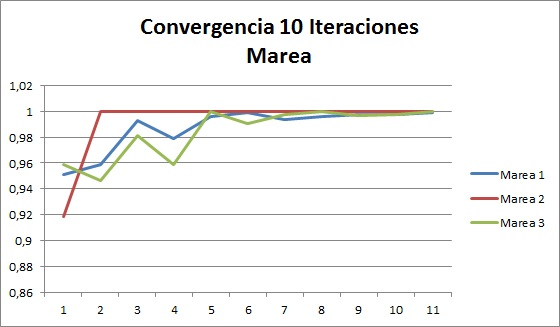
\includegraphics[scale=0.7]{figuras/graficos/Marea.jpg}
%  \caption {Marea. Convergencia en instancia Large para las 3 configuraciones.} 
%  \label{GraficaMarea}
% \end{center}
%\end{figure}

Sin nada más que referirnos, pasemos a observar una figura similar, pero correspondiente a la función Rastrigin. En este caso, 
no hace falta señalar que la convergencia hacia abajo se debe, a que es una función de minimización. No hay demasiado que 
destacar en esta figura, sólo un par de cosas:

\begin{itemize}
 \item La configuración 3 es la que se comporta mejor, de manera destacada en las 100 primeras iteraciones de Rastrigin. Por detrás 
 de ella iría la configuración 2 y finalmente la uno parece que es la peor.
 \item En este caso podemos ver lo anteriormente comentado, parece que la mayor convergencia es fruto del azar y 
 la probabilidad, puesto que las configuraciones 1 y 3 son la misma, pero es bastante probable, que al generar 50 mil individuos 
 saldrá unos mejores individuos que al generar 10 mil como ocurre en la configuración número 1.
\end{itemize}


%\begin{figure}[h]
%  \begin{center}
%  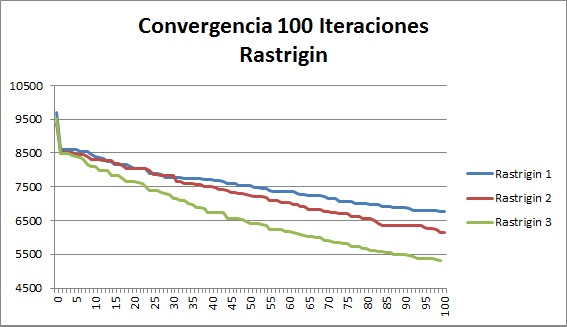
\includegraphics[scale=0.7]{figuras/graficos/Rastrigin.jpg}
%  \caption {Rastrigin. Convergencia en instancia Large para las 3 configuraciones.} 
%  \label{GraficaRastrigin}
% \end{center}
%\end{figure}


Por último, la Figura \ref{GraficaOneMax}, muestra la convergencia durante 300 iteraciones de la función OneMax, que cuenta 
los unos de un cromosoma binario, hasta maximizar este número. El  óptimo sería 512, que es el tamaño de la cadena elegido 
para observar los resultados.

\begin{itemize}
 \item El mejor comportamiento es la configuración 3. Parece que aquí influye de nuevo el número de individuos de la población. 
 Llega al óptimo casi unas 20 iteraciones antes que sus competidores.
 \item El reemplazo generacional de la configuración 2 vemos que en un inicio de algoritmo puede no ser muy bueno si no hay buena 
 calidad en la población inicial, sin embargo observamos que la convergencia es constante, no como en el caso de la primera, que 
 tras un buen inicio, converge más lentamente hasta ser la última en alcanzar el óptimo. Quizás el hecho de la menor presión 
 de selección haya influido en esto.
\end{itemize}





No se han observado significativos cambios en los resultados utilizando los dos diferentes métodos de cruce que disponemos. 




\subsection{Análisis}
Una vez vistos los resultados, analizando las tablas de tiempos, ficheros de resultados y gráficas obtenidas 
podemos sacar las siguientes conclusiones:

\begin{itemize}
 \item \textbf{Limitación de Algunas instancias}. Algunas de las instancias, como era evidente no tienen memoria suficiente para realizar tareas complejas de cálculos. En 
 nuestro caso, ha quedado demostrado en las instancias micro que no ha podido resolver Rastrigin con la configuración 2 y 3, y 
 la small que no ha podido resolver la configuración 3 del mismo problema, ambas por falta de memoria, debido a que el problema 
 Rastrigin trabaja con un gran número de números reales de precisión doble lo que hace ocupar gran parte de la memoria disponible.
 \item \textbf{Beneficioso}. En los demás casos, la utilización del cloud computing ha sido favorable debido a que los tiempos que nos han dado 
 han sido muy parecidos, en muchos casos mejores, a los de nuestro pc, lo que lleva a pensar que para casos más complejos 
 se podrían comportar mejor.
 \item \textbf{Trabajo Paralelo en Instancias}. Otra ventaja ha sido, que, en el mismo tiempo que se han realizado las ejecuciones para nuestro entorno local, han sido 
 llevadas a cabo todas las ejecuciones en las seis instancias en la nube, ya que, las instancias han trabajado paralelamente y,
 lógicamente, sin influir unas con otras.
 \item \textbf{Selección}. Para el caso de la selección, en nuestro caso se ha comportado mejor la selección determinística por torneo, puesto que 
 los problemas que hemos tratado no son muy complejos, se ha llegado al óptimo relativamente rápido y no han requerido de una 
 amplía búsqueda ni en la salida de grandes óptimos locales, que son en los casos en los que la probabilística podría 
 resultar favorable. Podemos apreciar una cosa curiosa en la selección probabilística, y es que cuando se ha alcanzado el óptimo, 
 y en todas las iteraciones sea este el mejor individuo, hay alguna iteración en los que se genera uno peor a él y es seleccionado 
 como mejor, quedando una gráfica y tanto rara.
 \item \textbf{Reemplazamiento}. El reemplazamiento generacional depende mucho de las tasas de selección, cruce y mutación elegidas. 
 Si éstas son bajas, la población puede ir incluso decreciendo, pueso que la generación anterior es entera borrada y 
 la nueva contendrá menos individuos. Esto hace que su comportamiento sea ligeramente más rápido en estos casos. Sin embargo, 
 en nuestro problema ha resultado mejor el reemplazamiento de los nuevos individuos generados por los menos adaptados de la 
 generación anterior (Worst), quizás por la misma razón que antes en la selección, no son problemas suficientemente complejos 
 que requieran de una diversidad grande.
 \item \textbf{Cruce}. No se ha encontrado ningún resultado digno de mencionar en cuanto al cruce de uno o dos puntos. Por cuestiones 
 puramente teóricas, podemos decir que el de dos puntos puede dar más diversidad a la población, pero no se ha visto que esto 
 quede plasmado en nuestro estudio.
 \item \textbf{Mejorable}. Para muchos exigentes, esto no es suficiente, necesitan mejoras de tiempos evidentes y por ello se 
 ha propuesto una alternativa mejor con Map Reduce, que se verá en el capítulo posterior.
\end{itemize}

\section{Conclusiones y trabajo futuro}
\label{sec:conc}




El Cloud Computing ha llegado con mucha fuerza y todo hace indicar que viene para quedarse.  Hemos visto durante, 
la primera parte que son muchas más las ventajas que nos ofrece este modelo que los inconvenientes a los que nos podemos 
enfrentar.  

Todo proveedor de computación en la nube, nos ofrece una infraestructura que, a no ser que estemos en una gran empresa o 
seamos poseedores de superordenadores, no está a nuestro alcance y ello nos hace que instantáneamente podamos acceder 
a esos recursos y hacer uso de ellos de una forma rápida, sencilla y con un coste bajo.  Precisamente esta posibilidad hace que 
sea una tecnología verdaderamente interesante para el mundo científico e investigador, pues habitualmente en tareas como 
análisis financiero, meteorológico o bioinformática, entre otras muchas cosas, se trabaja con ingentes cantidades de datos 
que requieren de millones de cálculos en poco tiempo y precisan de mucho tiempo, pese a tener grandes centros de datos. 

Por ello en este trabajo se ha propuesto un pequeño estudio dentro del gran mundo que es la bioinformática, utilizando 
la infraestructura de Amazon, el mayor proveedor de Cloud Computing y mucho más configurable que Google App Engine,
para la ejecución y análisis de algoritmos genéticos básicos.  

Se ha implementado una pequeña librería para el diseño de algoritmos genéticos de forma secuencial y un completo manual para 
la ejecución de estos algoritmos en los servicios web de Amazon.  Las características más importantes de esta propuesta han sido:

\begin{itemize}
 \item \textbf{Extensibilidad:} Desde el primer momento de desarrollo se ha pretendido dotar a la librería de un carácter extensible, 
 abstrayendo todo lo posible los distintos elementos dentro de un AG con el uso de interfaces, herencia y demás 
 ventajas de un lenguaje como Java y facilitando el prototipado rápido de AGs  mediante la implementación de un número mínimo de 
 funciones.

 \item \textbf{Portabilidad}: La aplicación se encapsula en un fichero JAR que puede ser ejecutado en cualquier entorno anfitrión que 
 disponga de un compilador Java, independientemente de su sistema operativo. Esto se ha hecho así, porque el objetivo principal e
 era ver las ventajas de computación en la nube, y lo mejor era un sistema portable entre distintas instancias volátiles en 
 Amazon EC2.

 \item \textbf{Sencillez}: El objetivo principal del trabajo, era conocer un poco más distintas posibilidades de servicios de la 
 nube de Amazon y como facilita el análisis de datos  y no profundizar mucho en Algoritmos Genéticos, por esta razón se han 
 implementado tres funciones sencillas. El único conocimiento necesario para realizar las pruebas viene explicado detalladamente 
 en el documento adjunto o la documentación generada por cada proyecto.
 
 \item \textbf{Aprendizaje}: Este trabajo es válido tanto como para alguien quiera iniciarse en el conocimiento de los algoritmos 
 genéticos, como para alguien que quiere sentar las bases de Cloud Computing tener acceso a instancias virtuales en Amazon.
 
\end{itemize}


Una vez vistos hecho el análisis de los resultados de la versión secuencial surgió la posibilidad de buscar una alterantiva  
paralela para un algoritmo genético  e investigando se encontró la posibilidad de  usar MapReduce, por ello, se ha descrito 
teóricamente en que consiste este modelo y en concreto, la implementación por parte de  Hadoop, que es la 
más conocida. 


Para introducirnos en el mundo de Hadoop, se ha explicado como hacer una configuración pseudo-distribuida en nuestro pc para 
comenzar a escribir aplicaciones de este tipo. Como primer ejemplo de ello, se ha propuesto y explicado la 
implementación de un básico contador de frecuencias de palabras en un conjunto de archivos, 
que pese a ser sencillo, nos da una muestra del potencial de MapReduce y de la sencillez de su implementación.  


Como extensión se ha presentado una aproximación a un sistema capaz de adaptar la naturaleza intensiva en datos del modelo MapReduce con el carácter 
iterativo de un Algoritmo Genético, sentando las bases para construir un software que permita ejecutar de forma distribuida 
algoritmos genéticos paralelos tanto sobre clústers, como sobre el servicio que nos proporciona Amazon Elastic MapReduce.  


En líneas generales, se ha descrito el diseño y la implementación de AGs básicos tanto de forma secuencial  como paralela utilizando 
entornos secuenciales y de cloud computing con Amazon como proveedor, y se ha introducido al uso del Framework de Hadoop para el 
diseño de aplicaciones con MapReduce.


Por último, destacar que las pruebas realizadas con la batería de problemas elegida (``Rastrigin'', ``OneMAX'' y ``Marea'') arrojan 
resultados satisfactorios en cuanto a escalabilidad y tiempo, teniendo en cuenta además que nuestra computadora desde la que 
mandamos los trabajos no consume recurso alguno. 


\section*{Futuras líneas de trabajo}


Hasta el momento solo ha podido desarrollarse un modelo de cómo sería la implementación de un algoritmo genético paralelo 
usando MapReduce.  La principal línea de trabajo sería terminar la implementación de este modelo y hacer extensible 
las clases implementadas para la parte secuencial a la parte paralela.

Dentro de la línea seguida en el proyecto podemos contemplar otras alternativas que completarían el estudio del modelo de 
programación MapReduce:

\begin{itemize}
 \item Se podría investigar si compensa la generación inicial de individuos con una tarea MapReduce como propone \cite{Gen09}. 
Esto sería útil para utilizar poblaciones de gran tamaño ya que en este caso, tendría un costo inicial muy alto para el 
nodo maestro mientras los otros se encontrarían ociosos.
 \item Otro aspecto que podría ser estudiado es la definición de una clase personalizada InputFormat (la encargada de describir la 
especificación de los datos de entrada de un trabajo MapReduce) para poder configurar el número de tareas map a gusto del usuario.
\end{itemize}

En lo que engloba al Cloud Computing, hay varias opciones que me gustaría llevar a cabo:

\begin{itemize}
 \item Mover una aplicación a la nube, migrar sus datos, configurar una  instancia para que no sea volátil, contratando una ip estática  y que 
 ésta actúe como servidor, y montar una página web en ella. 
 \item Utilizar proveedores PaaS, como Windows Azure o Google App Engine para desarrollar un servicio en la web. 
\end{itemize}


En conclusión, prácticamente para cualquier cosa en Internet se puede usar el Cloud Computing o aprovecharse de él, sólo se ha visto 
una pequeña parte, pero hay mucha luz detrás de las nubes.


% Eh.. un poco escaso, ?no?
\bibliographystyle{splncs}
\bibliography{cloudproject}
\end{document}
